% OCEANS 2027 Aberdeen submission draft.
% Compile: pdflatex with IEEEtran.cls (standard in TeX Live / Overleaf).
% Submission portal opens 2026-10-01; abstract/paper deadline 2027-01-15.
% All detection numbers from docs/competitions/public-floatwaste-benchmark.md
% (single source of truth). Do NOT cite numbers outside that file.
\documentclass[conference]{IEEEtran}
\IEEEoverridecommandlockouts
\usepackage{cite}
\usepackage{amsmath,amssymb,amsfonts}
\usepackage{booktabs}
\usepackage{graphicx}
\usepackage{textcomp}
\usepackage{xcolor}
\usepackage{tikz}
\usetikzlibrary{positioning,arrows.meta}
\usepackage{url}

% TODO before submission: complete co-author list, emails, and any funding note.
\newcommand{\todo}[1]{\textcolor{red}{[TODO: #1]}}

\begin{document}

\title{Oceanus: An Auditable LLM Governance Agent for Marine Debris
Response in Aquaculture Zones}

\author{\IEEEauthorblockN{Yongxiang Li\todo{complete co-author list}}
\IEEEauthorblockA{\todo{school/department}, Fuzhou Institute of Technology,
Fuzhou, China\\
\todo{email addresses}}}

\maketitle

\begin{abstract}
Coastal aquaculture zones face chronic floating debris---expanded-polystyrene
buoy fragments, discarded fishing gear, and feed bags---that existing
technology already ``sees'': video monitoring networks detect it and cleanup
robots collect it. The bottleneck has moved from perception to decision: who
decides what to clean, on what legal basis, with what oversight, and with what
audit trail after the fact. We present Oceanus, a deployed-software governance
agent for aquaculture-zone marine debris response that makes the decision
layer itself accountable. The agent plans response actions, invokes tools,
is intercepted by a policy guard on out-of-policy actions, routes them to
human approval, dispatches a MQTT-connected surface robot with three-bin
sorting, and replays every decision from an audit log that binds each
conclusion to versioned regulatory evidence. Domain knowledge is organized as
an evidence-audited ontology---100 nodes and 200 relations over 27 registered
assets in the current version---in which every extracted node and relation
must carry a citation that verifies verbatim against the registered source
text (96\% of node names and 85\% of relations fully traceable). Perception
runs three interchangeable channels, including an open-vocabulary zero-shot
detector whose vocabulary can be extended on site without retraining; on the
public SC-FloatWaste benchmark (official validation split as untouched test,
400 images, 3 regions), the zero-shot channel reaches 0.143 mAP@0.5 with
precision-oriented behaviour, while a YOLO11s channel fine-tuned on 600
training images reaches 0.514 mAP@0.5 (3.6$\times$), with cross-region
generalization reported per region. All tools and knowledge are exposed to
external agents through the Model Context Protocol (21 read-only tools). We
report honest boundaries throughout: benchmark accuracy is not field
accuracy, and the approval workflow has not yet been exercised by a real
authority.
\end{abstract}

\begin{IEEEkeywords}
marine debris, governance agents, LLM agents, auditability,
human-in-the-loop, open-vocabulary detection, Model Context Protocol
\end{IEEEkeywords}

\section{Introduction}
Aquaculture zones along the Chinese coast accumulate floating debris at a
rate that makes manual patrols uneconomical: expanded-polystyrene (EPS) buoy
fragments from rafts, derelict fishing gear, and feed bags. The technology
landscape already covers the two ends of the problem. Video monitoring
networks---deployed at city and county scale since at least
2020---detect and quantify debris. Cleanup platforms such as WasteShark and
Clearbot collect it, one machine at a time. What is missing is the layer
between: a decision process that turns detections into dispatched,
legally grounded, humanly approved cleanup actions---and that can be
audited afterwards.

This gap is not a perception problem but an accountability problem. A
governance decision (``dispatch the robot to grid cell X because debris type
Y exceeds threshold Z under regulation W'') must cite its basis, survive
challenge, and be replayable. Large language model (LLM) agents are now
capable of the planning and tool-use parts, but exactly their fluency makes
auditability non-negotiable: an agent that explains itself convincingly is
not the same as an agent whose every claim traces to registered evidence.

Oceanus is a software system built around this observation. Its contribution
is not a better detector but a decision loop with accountability as a design
constraint:

\begin{enumerate}
\item \textbf{An auditable decision pipeline}
(Sect.~\ref{sec:pipeline}): planning $\to$ tool invocation $\to$ policy
guard $\to$ human approval $\to$ dispatch $\to$ audit replay, with every
decision bound to versioned knowledge assets, an ontology version, and a
policy version.
\item \textbf{Evidence-audited domain knowledge} (Sect.~\ref{sec:knowledge}):
a versioned ontology in which every node and relation extracted by rules or
an LLM must cite a passage that verifies verbatim against registered source
documents; a deterministic audit reports traceability rates.
\item \textbf{Interchangeable perception, honestly measured}
(Sect.~\ref{sec:perception}): three channels---a temporal OpenCV channel for
production, an open-vocabulary zero-shot channel whose vocabulary extends on
site without retraining or restart, and a supervised channel---evaluated on a
public benchmark with region-level reporting and negative results reported
as such.
\item \textbf{Standard-protocol interoperability} (Sect.~\ref{sec:knowledge}):
knowledge, retrieval, events, and work orders are exposed as 21 read-only
tools over the Model Context Protocol (MCP), so external agents can use the
same evidence-backed capabilities.
\end{enumerate}

\section{Related Work}
\textbf{Marine debris and monitoring.} Debris harms marine life across
taxa~\cite{gall2015}, and coastal governments have deployed video
monitoring and cleanup programmes for years; public tenders and municipal
systems at city scale have existed in China since 2020. Commercial cleanup
platforms---WasteShark~\cite{wasteshark}, Clearbot~\cite{clearbot}---are
single-machine products with onboard collection. Both strands treat
decision-making as a human task. Oceanus keeps both ends replaceable---
cameras and robots are endpoints---and concentrates the contribution in
the decision layer. Compared on price and capability
(Table~\ref{tab:compare}), single-machine products leave the governance
workflow unbuilt.

\textbf{LLM agents, tool use, and auditability.} LLM-based autonomous
agents~\cite{agentsurvey} couple planners to tool APIs; retrieval-augmented
generation~\cite{lewis} grounds answers in retrieved text. Our concern is
not planner design but the guardrails around it: deterministic policy
checks before execution, human approval for out-of-policy actions---
a human-in-the-loop pattern with long precedent in interactive machine
learning~\cite{hitl}---and replayable traces that bind each step to
versioned knowledge. \textbf{Open-vocabulary detection.} YOLO-World
\cite{yoloworld} detects arbitrary text prompts zero-shot; supervised
detectors such as YOLO11~\cite{yolo11} lead in accuracy when training data
exists. We use the former as an operational capability (inspectors name a
new debris class on site) and measure its real accuracy profile on a
public benchmark~\cite{scfloatwaste} rather than assuming it.

\begin{table}[t]
\caption{Qualitative comparison with cleanup platforms. WasteShark list
price from public listing (approx.\ USD 23,600), converted at 7.2 CNY/USD.}
\label{tab:compare}
\centering
\small
\begin{tabular}{p{1.9cm}p{2.7cm}p{2.9cm}}
\toprule
 & Cleanup platforms & Oceanus \\
\midrule
Form factor & single machine & auditable agent + replaceable endpoints \\
Decision & manual & plan $\to$ guard $\to$ approve $\to$ execute $\to$ replay \\
New classes & product change & add a vocabulary word on site \\
Basis & none & versioned regulatory evidence chain \\
Sorting & none / single bay & three-bin coarse sorting + shore-side fine sorting \\
Indicative cost & $\sim$USD 23.6k (WasteShark) & commodity hardware, open stack \\
\bottomrule
\end{tabular}
\end{table}

\textbf{LLM agents and tool use.} Agent frameworks couple LLM planners to
tool APIs; our concern is not planner design but the guardrails around it:
policy checks before execution, human approval for out-of-policy actions,
and replayable traces. \textbf{Auditability and grounding.} Binding
generated text to retrieved evidence is studied as attribution and
grounding; we apply the same discipline to ontology construction, where the
audit unit is a triple plus its citation. \textbf{Open-vocabulary
detection.} YOLO-World and similar models detect arbitrary text prompts
zero-shot; we use this as an operational capability (inspectors can name a
new debris class on site) and measure its real accuracy profile on a public
benchmark rather than assuming it.

\section{System Architecture}
Oceanus organizes a three-tier loop: (i) \emph{perception}---shore-based
cameras with an edge box running detection; (ii) \emph{decision}---the
governance agent on the data platform; (iii) \emph{execution}---a surface
robot connected over MQTT, with three-bin coarse sorting on board and
shore-side fine sorting. Data flows back from operations into heat maps,
work orders, and reports, closing the governance loop. The software
comprises five subsystems: edge sensing, onboard robot software, the data
platform (FastAPI, PostgreSQL with PostGIS, Redis, EMQX MQTT, MinIO,
go2rtc streaming, Vue~3 front end), a training pipeline, and an inference
service. The robot is a replaceable MQTT work endpoint: with it offline, the
platform still completes event understanding, planning, guard checks,
approval, dispatch, audit, and replay---the configuration under which the
system currently runs.

\begin{figure*}[t]
\centering
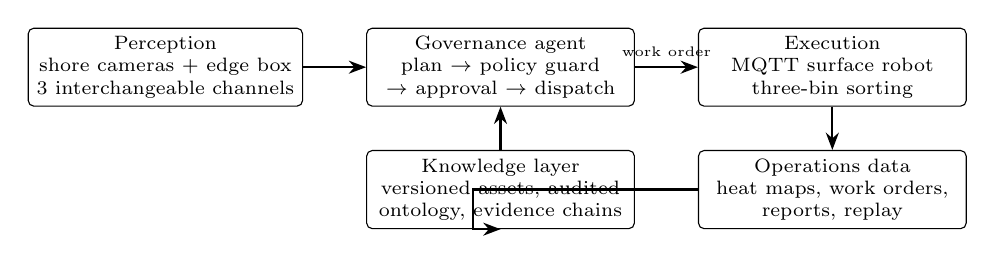
\begin{tikzpicture}[
  font=\scriptsize,
  box/.style={draw, rounded corners=2pt, align=center, inner sep=3pt,
    minimum width=3.4cm, minimum height=0.78cm},
  arr/.style={-{Stealth[length=2.2mm]}, thick},
]
\node[box] (edge) {Perception\\shore cameras + edge box\\3 interchangeable channels};
\node[box, right=0.8cm of edge] (agent) {Governance agent\\plan $\to$ policy guard\\$\to$ approval $\to$ dispatch};
\node[box, right=0.8cm of agent] (robot) {Execution\\MQTT surface robot\\three-bin sorting};
\node[box, below=0.55cm of agent] (kb) {Knowledge layer\\versioned assets, audited\\ontology, evidence chains};
\node[box, below=0.55cm of robot] (ops) {Operations data\\heat maps, work orders,\\reports, replay};
\draw[arr] (edge) -- (agent);
\draw[arr] (agent) -- (robot) node[midway, above, font=\tiny]{work order};
\draw[arr] (robot) -- (ops);
\draw[arr] (ops.west) -| ([xshift=-0.35cm]kb.south) -- (kb.south);
\draw[arr] (kb) -- (agent);
\end{tikzpicture}
\caption{Three-tier governance loop. The knowledge layer binds every agent
decision to versioned evidence; operations data flows back into knowledge
and reporting.}
\label{fig:arch}
\end{figure*}

\section{The Auditable Decision Pipeline}
\label{sec:pipeline}

\begin{figure}[t]
\centering
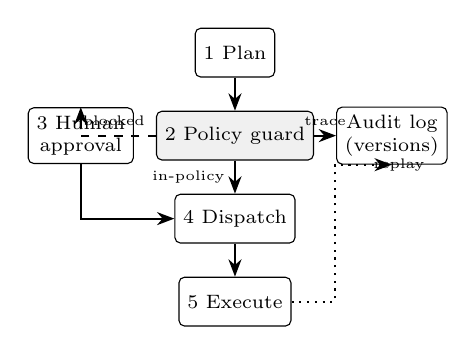
\begin{tikzpicture}[
  font=\scriptsize,
  node distance=0.42cm and 0.42cm,
  st/.style={draw, rounded corners=2pt, align=center, inner sep=3pt,
    minimum height=0.62cm},
  gate/.style={draw, rounded corners=2pt, align=center, inner sep=3pt,
    minimum height=0.62cm, fill=black!6},
  arr/.style={-{Stealth[length=2.2mm]}, thick},
  rej/.style={-{Stealth[length=2.2mm]}, thick, dashed},
]
\node[st] (plan) {1 Plan};
\node[gate, below=of plan] (guard) {2 Policy guard};
\node[st, below=of guard] (dispatch) {4 Dispatch};
\node[st, below=of dispatch] (exec) {5 Execute};
\node[st, left=0.28cm of guard] (approve) {3 Human\\approval};
\node[st, right=0.28cm of guard] (audit) {Audit log\\(versions)};
\draw[arr] (plan) -- (guard);
\draw[arr] (guard) -- node[left, font=\tiny]{in-policy} (dispatch);
\draw[rej] (guard.west) -| node[above, pos=0.28, font=\tiny]{blocked} (approve.north);
\draw[arr] (approve.south) |- (dispatch.west);
\draw[arr] (dispatch) -- (exec);
\draw[arr] (guard.east) -- node[above, font=\tiny]{trace} (audit.west);
\draw[arr, dotted] (exec.east) -- ++(0.55,0) |- node[right, pos=0.75, font=\tiny]{replay} (audit.south);
\end{tikzpicture}
\caption{The accountability envelope around every response action. The
policy guard blocks out-of-policy plans before execution; blocked or
high-impact actions require human approval; every step is logged with
knowledge-asset, ontology, and policy versions for later replay.}
\label{fig:pipeline}
\end{figure}
The agent runtime executes a fixed accountability envelope around every
response action (Fig.~\ref{fig:pipeline}):

\begin{enumerate}
\item \textbf{Planning.} Given an event (detection cluster, location,
time), the agent plans a response using registered tools.
\item \textbf{Policy guard.} Before execution, planned actions pass a
deterministic policy check (scope, budget, zone restrictions, action-type
rules). Out-of-policy plans are blocked, not executed.
\item \textbf{Human approval.} Blocked or high-impact actions route to an
approval queue; nothing executes until a human approves.
\item \textbf{Dispatch and execution.} Approved actions dispatch work
orders (MQTT to the robot when online; queued otherwise).
\item \textbf{Audit replay.} Every step---plan, guard verdict, approval,
dispatch, outcome---is logged with the knowledge-asset versions, ontology
version, and policy version that were live at decision time, so any past
decision can be reconstructed exactly.
\end{enumerate}

The knowledge-backed question-answering layer follows the same discipline:
retrieval first, then generation with inline numbered citations; when
evidence is insufficient the system states a refusal instead of generating,
and if the LLM call fails it degrades to presenting the raw evidence list.
Refusal is decided on \emph{evidence coverage}, not retrieval score; we
later show why (score-based abstention is configuration-fragile on small
regulatory corpora).

\section{Perception Channels and Public-Benchmark Evaluation}
\label{sec:perception}

\subsection{Channels}
Three interchangeable channels share one interface: (i) a production
OpenCV channel (background modeling plus color/shape rules) that depends on
continuous frames, runs on CPU, and is tuned per site; (ii) an
\emph{open-vocabulary} zero-shot channel (YOLO-World) whose vocabulary is a
runtime word list---an inspector can name ``foam buoy fragment'' on site and
the detector picks it up without retraining or restart; and (iii) a
supervised YOLO11s channel for accuracy when training data exists. The
channels are compared side by side in the product UI under a
\texttt{/vision-compare} view so their operating regimes are visible rather
than claimed.

\begin{table*}[t]
\caption{Main results on the untouched test split (400 images, 1,490 boxes,
3 regions, single class ``litter''). AP computed with all-point
interpolation at model-side confidence floor 0.001 (not the operating
threshold).}
\label{tab:main}
\centering
\small
\begin{tabular}{lrrr}
\toprule
Channel & mAP@0.5 & mAP@50:95 & best F1 \\
\midrule
Zero-shot (YOLO-World~\cite{yoloworld}, imgsz 960) & 0.1432 & 0.0930 & 0.2702 \\
Zero-shot (YOLO-World, imgsz 1280) & 0.1155 & 0.0744 & 0.2417 \\
Fine-tuned (YOLO11s~\cite{yolo11}, imgsz 1280) & \textbf{0.5135} & \textbf{0.3444} &
\textbf{0.5376} \\
\bottomrule
\end{tabular}
\end{table*}

\subsection{Evaluation protocol}
Static-image accuracy is measured on the public SC-FloatWaste benchmark
(CC~BY~4.0; 7,906 images, 27,583 boxes, 25 fine classes across three
regions: Indonesia/Citarum, Australia NSW, Australia Tasmania). We use the
\emph{official} train/val split, which the dataset publisher declares
disjoint: the official validation split (400 images, 1,490 boxes) is our
untouched test set; 600 official-train images from Indonesia form the
training set and 172 a validation set. Manifest selection is deterministic
(within-region filename order; no random splits, which would leak adjacent
video frames). Model selection uses only the validation split (best
validation mAP@0.5 at epoch 48); the test set was never used for any tuning
choice. The zero-shot vocabulary was frozen in code \emph{before} the
benchmark was adopted (plastic bottle, plastic waste, garbage, fishing net,
foam debris, marine debris, discarded shoe). Every metric JSON records
commands, dates, weight hashes, manifests, and claim boundaries.

\begin{table}[t]
\caption{Per-region results (mAP@0.5). Training used Indonesia only; NSW
and Tasmania are fully cross-domain.}
\label{tab:regions}
\centering
\small
\begin{tabular}{lrrr}
\toprule
Region (images / boxes) & Zero-shot & Fine-tuned & Domain \\
\midrule
Indonesia (90 / 850) & 0.1299 & \textbf{0.7229} & training \\
NSW (164 / 204) & 0.2105 & \textbf{0.3341} & cross \\
Tasmania (146 / 436) & 0.2408 & \textbf{0.4029} & cross \\
\midrule
All (400 / 1,490) & 0.1432 & \textbf{0.5135} & --- \\
\bottomrule
\end{tabular}
\end{table}

\subsection{Findings, including negative ones}
Table~\ref{tab:main} and Table~\ref{tab:regions} support four findings.
(1)~Supervised training pays: fine-tuned YOLO11s lifts mAP@0.5 from 0.143
to 0.514 (3.6$\times$; best F1 0.5376 at precision 0.5665 / recall 0.5114).
(2)~The zero-shot channel is precision-oriented: at confidence 0.05 it
holds precision 0.5054 at recall 0.0631, and its dominant failure mode is
misses, not false alarms (Indonesia: 589 detections against 850 ground-truth
boxes). This is the accuracy profile of a \emph{supplementary on-site
extension channel}, not a primary alarm channel---which is exactly how the
product deploys it. (3)~Raising input resolution \emph{lowered} zero-shot AP
(0.143$\to$0.116): higher resolution produced more low-confidence false
positives, so operating points must be calibrated per channel. (4)~Longer
training traded cross-domain generalization for in-domain accuracy: an
early checkpoint scored 0.443 on NSW while the fully-trained model scores
0.334 there (in-domain rose 0.627$\to$0.723). Domain adaptation needs
multi-region data, not more epochs---one reason local data collection is
prioritized over public-benchmark tuning.

\subsection{Honest boundaries}
These are third-party public-benchmark numbers on river and urban waterway
imagery. They are \emph{not} field validation in the target aquaculture
zones, whose EPS-dominant debris, sea-state, and lighting distributions
differ; the local test set is still empty pending a collection campaign, and
no on-site accuracy claim is made. The production OpenCV channel requires
continuous frames and is not evaluable on static-image benchmarks; its
76\% figure in project materials is a temporal false-alarm suppression rate
on a different pipeline and must not be mixed with the benchmark numbers.

\section{Knowledge Assets and Interoperability}
\label{sec:knowledge}

\subsection{Versioned assets and evidence-audited ontology}
Documents, tables, images, events, telemetry, and datasets register as
immutable-versioned assets. A domain ontology (current published version:
100 nodes, 200 relations over 27 assets, primarily marine dumping
regulations from the national environmental authority) is built through
candidate extraction $\to$ human review $\to$ publish. The auditable-by-
construction invariant: every node and relation carries at least one
evidence citation $\langle$asset, version, snippet$\rangle$. A
deterministic audit re-verifies each snippet verbatim against the registered
text and checks endpoint occurrence in citing documents: currently 89.9\%
of citations verify verbatim (302/336), 90\% of relation endpoints are
traceable, 85\% of relations are fully traceable, and 96\% of node names
occur in their source document. Non-verbatim citations feed the review
queue rather than being silently accepted. Retrieval over these assets is
multi-hop (ontology graph expansion) and every decision stores its evidence
chain---asset versions, ontology version, policy version---for replay. On a
306-question type-stratified benchmark over this corpus (title, entity,
two-hop, and refusal queries, deterministically constructed from the
ontology and asset tables), the deployed graph-expanded retriever reaches
98.3\% hit@5 on two-hop queries and 93.0\% on entity queries, and a
two-system rule router that sends title-coverage queries to plain BM25 and
everything else to the graph retriever attains 97.0\% overall hit@5,
statistically matching a per-query-type oracle---while no configuration's
retrieval scores separate answerable from out-of-domain queries, which is
why the QA layer abstains on evidence coverage rather than score.

The question-answering workbench enforces the same discipline at the user
interface: answers carry inline numbered citations whose badges locate the
grounding evidence card (including hop paths and asset-version references);
when retrieved evidence is insufficient the interface shows an explicit
refusal banner instead of a generated answer, and if the LLM call itself
fails the system degrades to presenting the raw evidence list. Refusal is
thus a first-class output, not an error path.

\subsection{Deployment status}
The decision-loop software and the MCP service run today as a single-node
cloud deployment: a FastAPI backend with PostgreSQL/PostGIS, Redis, EMQX
and MinIO, fronted by the MCP server (stdio and Streamable HTTP). The
21-tool read-only surface has been exercised end-to-end by an external
hosted agent platform: real question-answering calls through knowledge
search and event tools completed successfully, with server-side logs
matching the platform's call traces step by step. The robot remains a
replaceable MQTT endpoint (offline in the current configuration); no field
campaign has yet been run, so no on-site accuracy or cleanup-effectiveness
claim is made anywhere in this paper.

\subsection{MCP interoperability}
The same capabilities are exposed to external agents through the Model
Context Protocol~\cite{mcp}: 21 read-only tools (Table~\ref{tab:mcp}) over
stdio or Streamable HTTP, with write tools disabled unless explicitly
enabled. Outbound calls authenticate with a dedicated service account and
refresh tokens before expiry; inbound HTTP uses a bearer token. Five
reusable workflow skills ship with the server. Any MCP-capable agent can
therefore pose questions and receive citation-backed answers from the same
versioned evidence the governance decisions use---interoperability without
giving up the audit chain.

\begin{table}[t]
\caption{The 21 read-only MCP tools by category (write tools exist but are
disabled unless explicitly enabled).}
\label{tab:mcp}
\centering
\small
\begin{tabular}{lp{5.1cm}}
\toprule
Category ($n$) & Tools \\
\midrule
Knowledge (7) & \texttt{knowledge\_} prefix: \texttt{list\_assets},
\texttt{asset\_detail}, \texttt{list\_ontology\_versions},
\texttt{ontology\_version\_detail}, \texttt{list\_ontology\_nodes},
\texttt{list\_ontology\_relations}, \texttt{search} \\
Decision evidence (2) & \texttt{knowledge\_list\_decisions},
\texttt{knowledge\_\allowbreak decision\_\allowbreak evidence} \\
Events (2) & \texttt{event\_list}, \texttt{event\_get} \\
Work orders (3) & \texttt{task\_list}, \texttt{task\_get},
\texttt{task\_ack\_history} \\
Dashboard (1) & \texttt{dashboard\_get} \\
Agent runtime (6) & \texttt{agent\_runtime\_status},
\texttt{agent\_list\_runs}, \texttt{agent\_run\_detail},
\texttt{agent\_run\_steps}, \texttt{agent\_list\_tools},
\texttt{agent\_list\_approvals} \\
\bottomrule
\end{tabular}
\end{table}

\section{Limitations}
(1)~No field deployment validation yet: perception accuracy is public-
benchmark only, and the aquaculture-zone test set is pending. (2)~The
approval workflow has not been exercised by a real authority; the human
role is currently project staff. (3)~The robot end is a replaceable MQTT
endpoint; end-to-end loops including physical collection have not been
validated at sea. (4)~The governance domain is one Chinese coastal county's
regulatory environment; the ontology and policy sets are locale-specific by
design. (5)~Open-vocabulary detection's low recall on cross-domain imagery
limits its role to a supplementary channel.

\section{Conclusion}
Oceanus moves marine debris response from ``can we see it?'' to ``can we
defend the decision?''. Its decision loop---plan, guard, approve, execute,
replay---binds every action to versioned, verbatim-verifiable evidence;
its knowledge layer is audited deterministically rather than trusted; its
perception is honestly measured on a public benchmark with negative results
reported; and everything is reachable by external agents over an open
protocol. The system runs today as decision-loop software with replaceable
perception and execution endpoints; the next step is the aquaculture-zone
field campaign that will turn public-benchmark accuracy into local
accuracy, under the same audit discipline.

%
% References
%
\begin{thebibliography}{10}

\bibitem{gall2015}
S.~C. Gall and R.~C. Thompson, ``The impact of debris on marine life,''
\emph{Marine Pollution Bulletin}, vol.~92, no.~1--2, pp. 170--179, 2015.

\bibitem{wasteshark}
RanMarine Technology, ``WasteShark aquadrone.'' [Online]. Available:
\url{https://www.ranmarine.io}

\bibitem{clearbot}
Clearbot, ``AI-powered autonomous cleaning boats.'' [Online]. Available:
\url{https://www.clearbot.org}

\bibitem{agentsurvey}
L.~Wang, C.~Ma, X.~Feng, Z.~Zhang, H.~Yang, J.~Zhang, Z.~Chen, J.~Tang,
X.~Chen, Y.~Lin, W.~X. Zhao, Z.~Wei, and J.-R. Wen, ``A survey on large
language model based autonomous agents,'' \emph{Frontiers of Computer
Science}, vol.~18, no.~6, 2024.

\bibitem{lewis}
P.~Lewis, E.~Perez, A.~Piktus \emph{et~al.}, ``Retrieval-augmented
generation for knowledge-intensive NLP tasks,'' in \emph{Proc. NeurIPS},
2020.

\bibitem{hitl}
X.~Wu, L.~Xiao, Y.~Wu, Q.~Z. Sheng, and S.~Wang, ``A survey on
human-in-the-loop machine learning,'' \emph{ACM Computing Surveys},
vol.~55, no.~13s, pp. 1--35, 2022.

\bibitem{yoloworld}
Y.~Xu, T.~Zhang, M.~Zhang, R.~Guo, G.~Tian, Y.~Zhang, X.~Hu, X.~Wang,
and J.~Dai, ``YOLO-World: Real-time open-vocabulary object detection,''
in \emph{Proc. IEEE/CVF CVPR}, 2024.

\bibitem{yolo11}
Ultralytics, ``YOLO11 object detection model,'' 2024. [Online]. Available:
\url{https://github.com/ultralytics/ultralytics}

\bibitem{scfloatwaste}
O.~Wu, ``SC-FloatWaste: A multi-region floating waste detection dataset,''
Zenodo, CC BY 4.0. doi: 10.5281/zenodo.21934286.

\bibitem{mcp}
Anthropic, ``Model Context Protocol,'' 2024. [Online]. Available:
\url{https://modelcontextprotocol.io}

\end{thebibliography}

\end{document}
